\documentclass[hyperref={colorlinks = true,linkcolor = black}]{beamer} 
\usepackage[MeX]{polski} 
\usepackage[utf8]{inputenc} 
\usetheme{Goettingen}
\usecolortheme{spruce}
\setbeamertemplate{caption}[numbered]
\usepackage{graphicx}
\usepackage{caption}
\usepackage{wrapfig}


\title{Zwierzęta}

\author{Maria Koren}

\begin{document}

\begin{frame}
\titlepage
\end{frame}

\begin{frame}{Definicja}
Zwierzęta (Animalia) – królestwo obejmujące wielokomórkowe organizmy cudzożywne o komórkach eukariotycznych, bez ściany komórkowej, w większości zdolne do aktywnego poruszania się. Są najbardziej zróżnicowanym gatunkowo królestwem organizmów.
\end{frame}

\begin{frame}{Gatunki zwierząt}
Jak piszą na stronie \cite{b1} isnieją następujące gatunki zwierząt:
\begin{enumerate} 
\item Ssaki 
\item Ptaki (przykłady ptaków są w tebeli \ref{tab:tabelka1})
\item Gady 
\item Płazy
\item Ryby  
\item Stawonogi
\end{enumerate}
\end{frame}

\begin{frame}{Rysunek}
Za najmniejsze foki uważa się nerpy. Osiągają długość do 130 cm i masę ciała maksymalną 110kg. „Największymi fokami” są mirungi, czyli słonie morskie, które też należą do tej rodziny. Samce, znacznie większe od samic, mogą przekraczać masę 3000 kg!  Wiecej na stronie \cite{b2}
\begin{figure}[h]
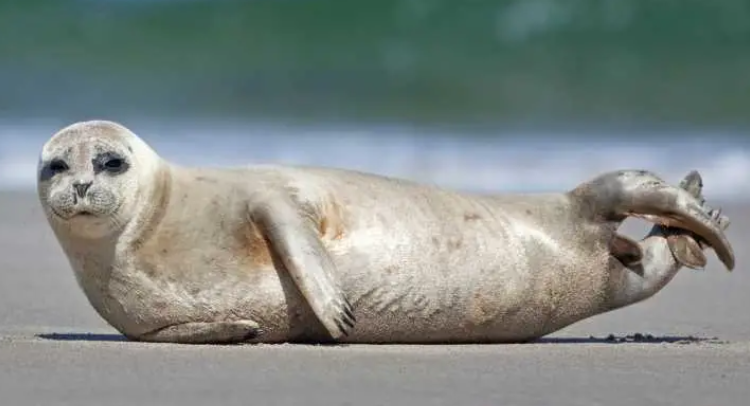
\includegraphics[scale=0.5]{foka.png}
\caption{Foka większe zdjęcie}
\label{fig:obr1}
\end{figure}
\end{frame}





\begin{frame}{Najbardziej egzotyczne zwierzęta}

Jeśli wierzyć stronie \cite{b3}, najbardziej egzotyczne zwierzęta to:
\begin{itemize}
  \item Jeż pigmejski, na zdjęciu \ref{fig:obr2}
  \item Fenek, na zdjęciu \ref{fig:obr3}
  \item Marmozeta, na zdjęciu \ref{fig:obr4}
  \item Skuns
  \item Kapibara, , na zdjęciu \ref{fig:obr5}
\end{itemize}

\end{frame}

\begin{frame}{Zdjęcia}

\begin{figure}[h]
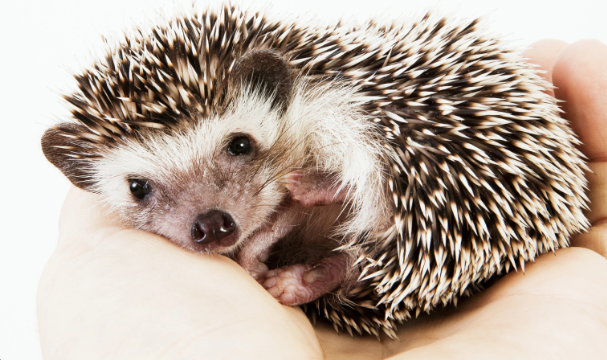
\includegraphics[scale=0.12]{jez.png}
\caption{Jeż pigmejski}
\label{fig:obr2}
\end{figure}

\begin{figure}[h]
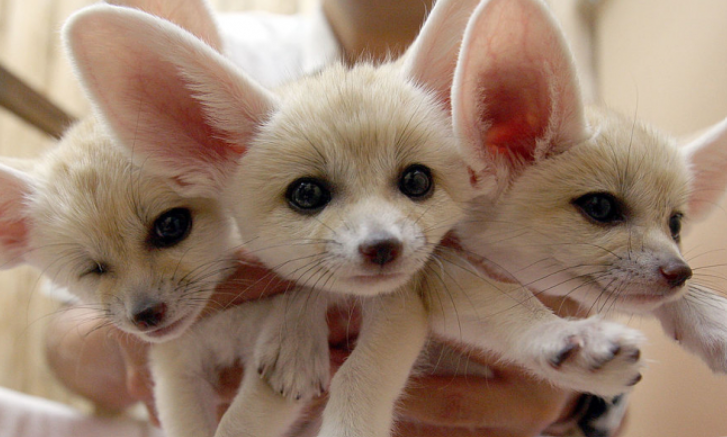
\includegraphics[scale=0.12]{fenek.png}
\caption{Fenek}
\label{fig:obr3}
\end{figure}

\begin{figure}[h]
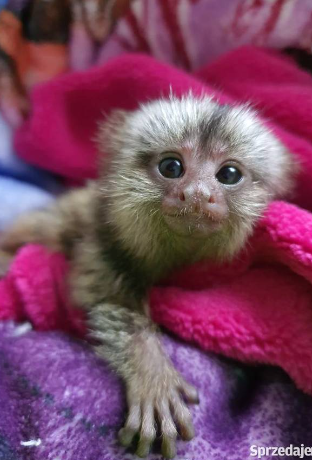
\includegraphics[scale=0.12]{marmozeta.png}
\caption{Marmozeta}
\label{fig:obr4}
\end{figure}

\begin{figure}[h]
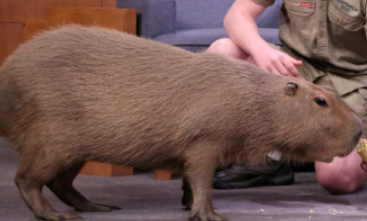
\includegraphics[scale=0.15]{kapibara.png}
\caption{Kapibara}
\label{fig:obr5}
\end{figure}
\end{frame}

\begin{frame}{Mrowka}
\begin{wrapfigure}{r}{0.6\textwidth}
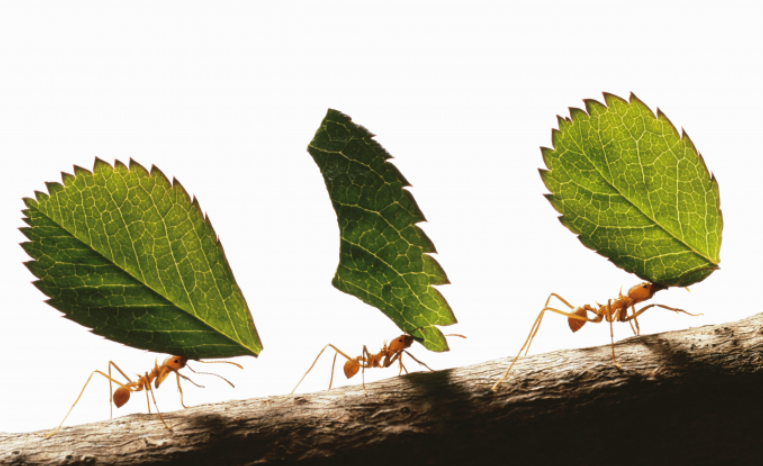
\includegraphics[scale=0.28]{mrowka.png}
\caption{Mrówka}
\label{fig:obr6}
\end{wrapfigure}
Kiedy \textbf{mrówka skalna} znajdzie nowe źródło pożywienia lub miejsce na gniazdo, prowadzi tam inną mrówkę za pomocą techniki zwanej biegiem tandemowym. Mrówka znająca trasę prowadzi nowicjusza wzdłuż niej, zatrzymując się po drodze, aby uczeń mógł zapamiętać każdy punkt orientacyjny. Nauczyciel polega na informacji zwrotnej od ucznia, który potwierdza, kiedy każda lekcja została przyswojona. Stuknięciem czułków daje nauczycielowi znać, że czas ruszać dalej
\end{frame}


\begin{frame}{Ptaki}
Typy ptaków (informacja ze strony \cite{b4})

\begin{table}[h]
\centering
\begin{tabular}{|c | c|}
\hline
 Ptaki wylatujący na zimę &  Ptaki  nie wylatujący na zimę \\
\hline
wilga & gołębie \\ \hline
słowik & kawki \\ \hline
jaskółka & sikorki \\ 
\hline
\end{tabular}
\caption{Tabela o ptakach}
\label{tab:tabelka1}
\end{table}

\end{frame}

\begin{frame}{Puszcza Białowieska}
Dużo zwierząt żyje w lasach. Tym samym w puszcze Białowieskiej

\begin{figure}[h]

\includegraphics{puszcza.png}
\caption{Logo puszczy}
\label{fig:obr7}
\end{figure}
\end{frame}

\begin{frame}{Żubr}
Najwiekszym ssakiem w puszczy jest żubr. 
\begin{figure}[h]
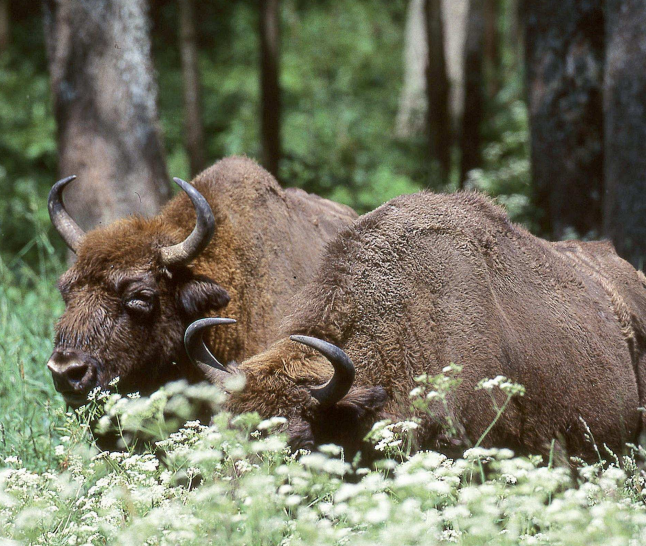
\includegraphics[scale=0.5]{zubr.png}
\caption{Żubr}
\label{fig:obr8}
\end{figure}
\end{frame}

\begin{frame}{Systematyka żubra}
Najpopolarniejszy gatunki żubra:
\begin{itemize}
  \item Bison bonasus bonasus
  \item Bison bonasus caucasus
  \item Bison bonasus hungarorum
\end{itemize}

\begin{figure}[h]
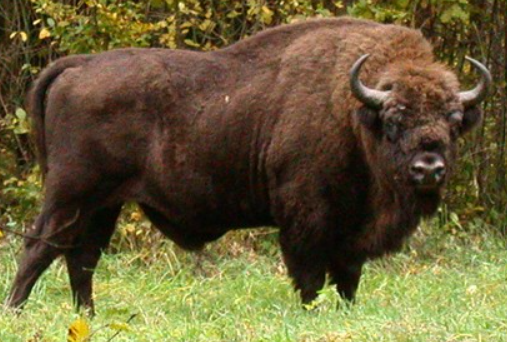
\includegraphics[scale=0.5]{zubr1.png}
\caption{Żubr}
\label{fig:obr9}
\end{figure}


\end{frame}



\begin{thebibliography}{4}
\bibitem{b1} https://www.zoo.zamosc.pl/page/3-gatunki-zwierzat
\bibitem{b2} https://zoo.wroclaw.pl/blog/2021/12/06/foka-pospolita/
\bibitem{b3} https://www.national-geographic.pl/artykul/9-egzotycznych-zwierzat-ktore-mozesz-trzymac-w-swoim-domu-zaskakujace-ciekawostki
\bibitem{b4} https://pl.wikibooks.org/wiki/Wikijunior:Zwierz%C4%99ta
\end{thebibliography}

\end{document}
